\begin{solution}
\begin{enumerate}
\item {[5 points]}  One way of coding the function is:

\lstinputlisting{initial.m}

The plot and code used to create it are below.

\begin{center}
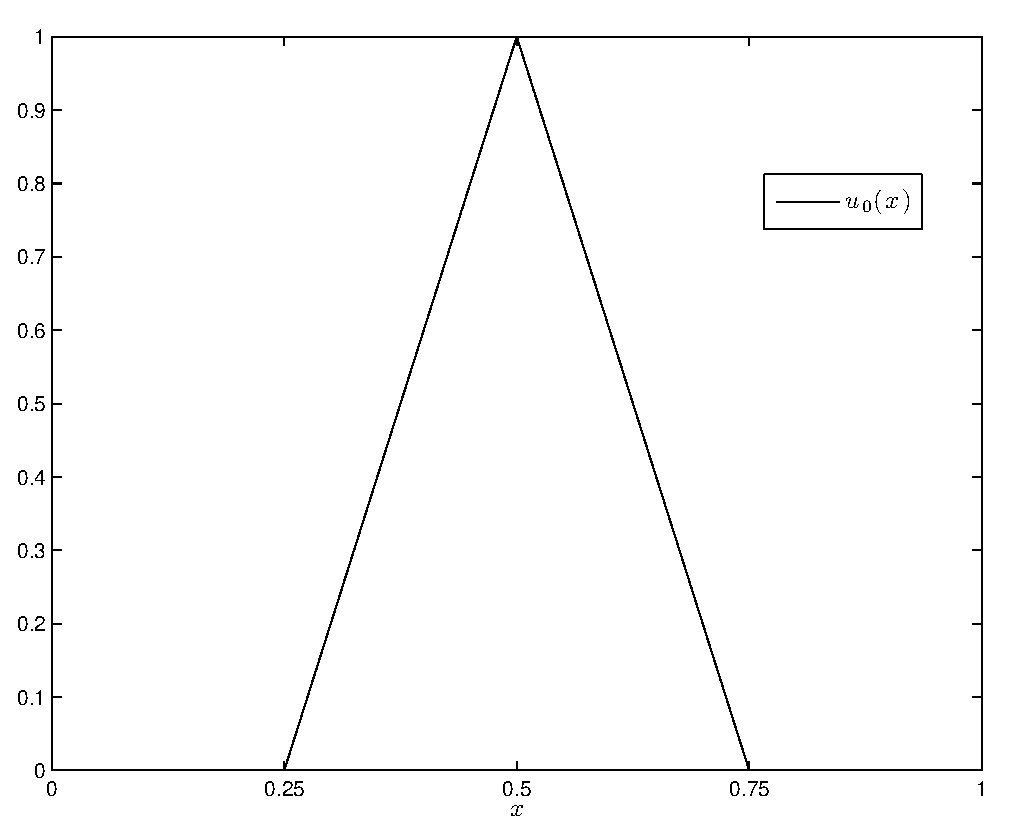
\includegraphics[scale=0.7]{hw49a.eps}
\end{center}

\lstinputlisting{HW49a.m}

\item {[10 points]} One way of coding the function is:

\lstinputlisting{initialinterpolant.m}

The plots and codes used to create them are below.

\begin{center}
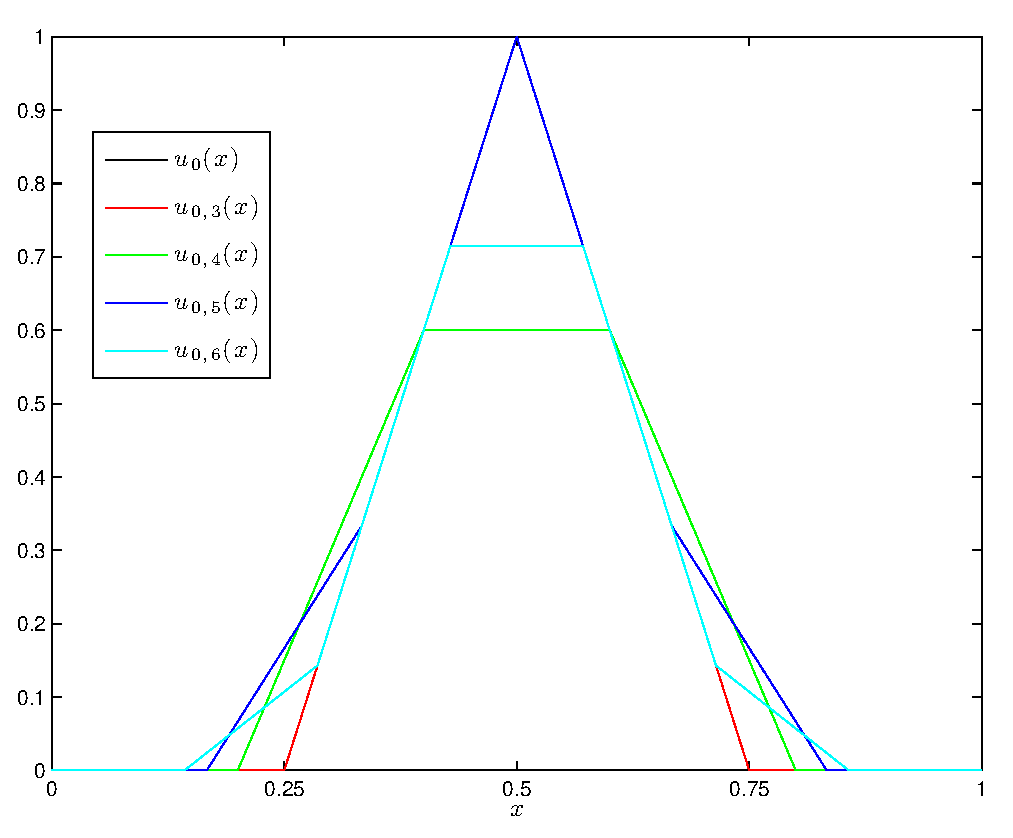
\includegraphics[scale=0.7]{hw49b1.eps}
\end{center}

\begin{center}
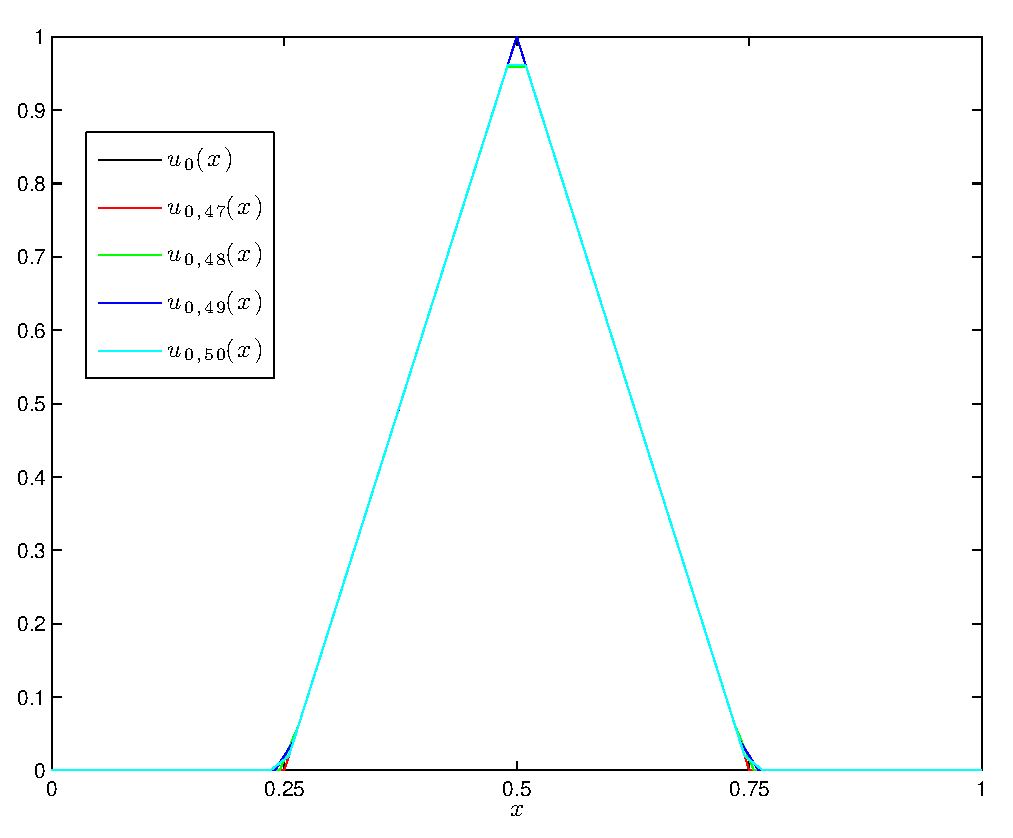
\includegraphics[scale=0.7]{hw49b2.eps}
\end{center}

\lstinputlisting{HW49b.m}

\item {[10 points]} When $N=3$ and $N=47$, $\displaystyle{\max_{x\in[0,1]}|u_0(x)-u_{0,N}(x)|}$ is smallest since $\displaystyle{\max_{x\in[0,1]}|u_0(x)-u_{0,N}(x)|}=0$ because $u_0=u_{0,N}$. From the definition of $u_0$ and the information about $V_N$ and $u_{0,N}$ given in the question, it follows that $u_0=u_{0,N}$ if and only if ${1 \over 4},{1 \over 2},{3 \over 4}\in\{x_0,x_1,\ldots x_{N+1}\}$. Now, $jh={j \over N+1}$, and so $jh={1 \over 4}$ when $j={N+1 \over 4}$. If $j={N+1 \over 4}$ then $0<j<N+1$ but in order for $jh\in\{x_0,x_1,\ldots x_{N+1}\}$, in addition, $j$ must be an integer. In order for this to be the case $N+1$ must be divisible by $4$ and so we can conclude that ${1 \over 4}\in\{x_0,x_1,\ldots x_{N+1}\}$ if and only if $N=4m-1$ where $m$ is a positive integer. Moreover, for such an $N$, $0<m<N+1$, $0<2m<N+1$ and $0<3m<N+1$ and $x_m={m \over 4m}={1 \over 4}$, $x_{2m}={2m \over 4m}={1 \over 2}$, and $x_{3m}={3m \over 4m}={3 \over 4}$. Consequently, $u_0=u_{0,N}$ if and only if
\[
N=4m-1
\]
where $m$ is a positive integer. For this reason, $u_0=u_{0,N}$ and hence $\displaystyle{\max_{x\in[0,1]}|u_0(x)-u_{0,N}(x)|}=0$ when $N=3$ and $N=47$ but $u_0\ne u_{0,N}$ and hence $\displaystyle{\max_{x\in[0,1]}|u_0(x)-u_{0,N}(x)|}\ne0$ when $N=4,5,6,48,49,50$.
\end{enumerate}
\end{solution}